\documentclass[a4paper]{article}
\usepackage[top=1in, bottom=1.25in, left=1.25in, right=1.25in]{geometry}


\usepackage{amsmath}
\usepackage{amssymb}
\usepackage{graphicx}
\usepackage[utf8]{inputenc}
 
\usepackage{amsthm}
\usepackage{enumitem}   
\usepackage{listings}

\lstset{
  breaklines=true,
  numbers=left,
  language=Python
}

\begin{document}

%% Title, authors and addresses

\title{Brain Inspired Computing - Problem Set 1}

\author{Sven Bordukat, Paul Meehan}

\date{\today}

\maketitle

\section*{Exercise 1}
\begin{itemize}
\item[a)]
As there are approximately $10^{11}$ neurons in the brain, each firing at around
1 Hz, and the total energy use is 20 W, we calculate the energy use per neuron:
\begin{align*}
    E_{spike} &= \frac{20 J/s}{10^{11}*1/s}\\
    &= 2 * 10^{-10} J
\end{align*}

$10^{15}$ synapses means $10^{4}$ synapses per neuron. This results in
\begin{align*}
    E_{event} &= \frac{2*10^{-10} J}{10^{4}}\\
    &= 2*10^{-14} J
\end{align*}

\item[b)]
As the time is 1 second and the neurons fire at 1 Hz, we have $1.23*10^9$
action potentials and $6*10^3*1.23*10^9=7.38*10^{12}$ synaptic events.
This gives us
\begin{align*}
    E_{spike} &= \frac{12.6*40*60*10^6 J}{1.23*10^9}\\
    &= 24.6J \\
    E_{event} &= \frac{12.6*40*60*10^6 J}{7.38*10^{12}}\\
    &= 4.1*10^{-3}J\\
\end{align*}

\item[c)]
In order to scale the system to the human brain, the number of neurons as well
as the number of synapses would need to be scaled by approximately 2 orders of
magnitude. This is equivalent to a number of computers $K\approx100$. This would
result in about 1.26GW of power usage.
\item[d)]
As the system performs the equivalent of 1 second in 40 minutes, the power consumption
is $40*60*1.26GW=3.024TW$. This system requires $3.024TW/1.78GW\approx1700$ nuclear
power plants to power it.

\end{itemize}

\section*{Exercise 2}
Values for $I_0, g_L, C_m$ were selected in order to produce a nice result.
The timescale is not in any specific unit.
\begin{figure}[htbp]
    \centering
    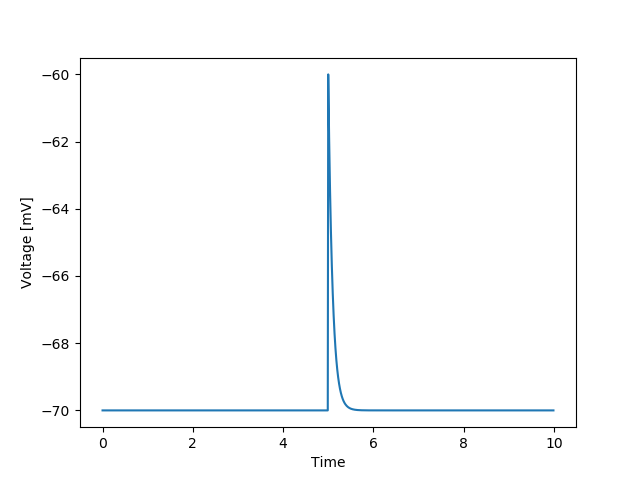
\includegraphics{a.png}
\caption{a)}
\end{figure}
\begin{figure}[htbp]
    \centering
    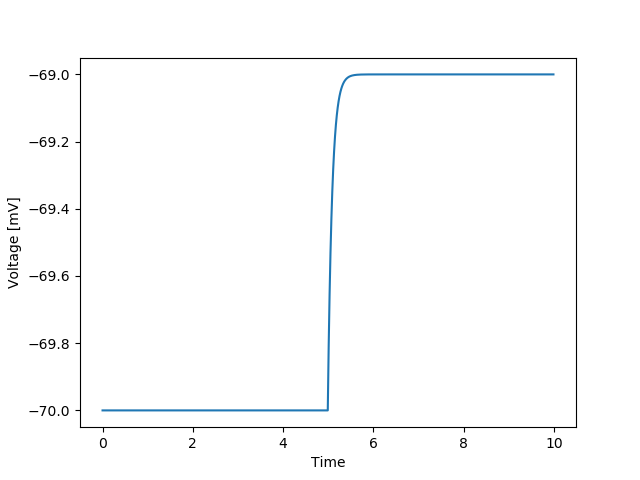
\includegraphics{b.png}
\caption{b)}
\end{figure}
\begin{figure}[htbp]
    \centering
    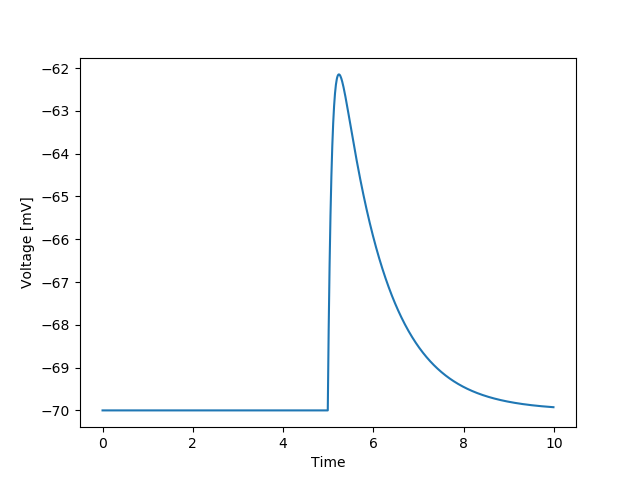
\includegraphics{c.png}
\caption{c)}
\end{figure}

\end{document}
